\chapter{How to Read a DNA Sequence}

\begin{kaichang}
Perhaps you have seen a small saliva-collection tube in the news. Spit into it, mail it to a company, and weeks later receive a report suggesting your ancestors' regions, whether you metabolize caffeine quickly or slowly, and which genetic variants you carry. There are other versions of this saliva trick: crime dramas identify suspects from one hair; a throat swab recently told you whether you carried a virus; a pregnant person's blood sample can screen for certain fetal chromosome abnormalities.

First guess how the mysterious machine reads DNA letters from saliva containing only shed cells and proteins. Does it really scan the DNA chain page by page?

We will open that black box. Reading DNA relies not on looking but on clever chemistry: first \textbf{copy}, then \textbf{separate}, and finally let DNA \textbf{leave its own clues} during synthesis.
\end{kaichang}

\textbf{Translator safety note:} Prenatal screening estimates risk rather than establishing a diagnosis. Discuss results and appropriate confirmation with a qualified clinician or genetic counselor before making pregnancy decisions. Consumer genetic reports likewise need clinical interpretation before medical use. See \href{https://content.govdelivery.com/accounts/USFDA/bulletins/3142524}{FDA prenatal-screening cautions} and \href{https://www.fda.gov/medical-devices/in-vitro-diagnostics/direct-consumer-tests}{FDA consumer-testing guidance}.

\section{Making More of a Target Segment: PCR}

Chapter 67 introduced DNA polymerase, the molecular copying machine. It follows an old strand as template and joins nucleotides one by one according to base-pairing rules, making a complementary strand. It works in a tube too, but there is a problem: saliva contains very little DNA, and the region of interest may be only a few hundred letters of one gene. Before finding a needle in an ocean, we must turn that needle into \textbf{ten billion copies}.

The method is polymerase chain reaction, or PCR. Its idea is surprisingly simple: if polymerase starts copying only from a particular point, give it a starting point of our choosing.

The target's beginning and end sequences are known. Chemists synthesize two short single-stranded DNA pieces, each about twenty letters, complementary to its ends. These \textbf{primers} act as labels saying ``start copying here.'' Put primers, polymerase, four nucleotide building blocks, and sample DNA in a small tube, then cycle through three temperatures:

\begin{itemize}[itemsep=2pt]
\item Heat to about $94\,^{\circ}\mathrm{C}$: thermal motion disrupts hydrogen bonds and separates the DNA strands, a step called denaturation.
\item Cool to about $55\,^{\circ}\mathrm{C}$: primers bind stably to their target positions, called annealing.
\item Warm to about $72\,^{\circ}\mathrm{C}$: polymerase extends from each primer along its template, called extension.
\end{itemize}

One cycle turns one target copy into two; another makes four, then eight. New strands from each cycle become templates in the next. Primers ensure that only the intervening segment is amplified, leaving billions of other genomic letters aside. This is PCR's selectivity: \textbf{it depends on base-pairing rules, not machine intelligence}. Primers bind only to complementary sequences.

\begin{qiaoliang}
PCR amplification is exponential: after $n$ cycles, the theoretical target count is $2^n$. Calculate $2^{10}\approx 10^3$, one thousand; $2^{20}\approx 10^{6}$, one million; and $2^{30}\approx 10^{9}$, one billion. Starting with even a few dozen target molecules, thirty cycles, about one or two hours in an automated instrument, yield tens of billions of copies, enough to detect. That explains how nucleic-acid tests can find a virus in a mouthful of sputum.

Real PCR does not double perfectly: enzymes sometimes fail, reagents run down, and abundant products interfere. At an average 1.8-fold increase per cycle, thirty cycles give $1.8^{30}\approx 4.6\times 10^{7}$, about one-twentieth of the ideal yield but still useful. Exponential growth remains powerful even with a smaller base: a few extra cycles compensate. Conversely, a tenfold starting difference produces exactly a tenfold final difference. PCR can therefore \textbf{count} original target molecules through quantitative PCR, for example to estimate viral infection severity.
\end{qiaoliang}

\textbf{Translator safety note:} A PCR result or cycle-threshold value alone does not establish how ill or infectious someone is. Interpretation depends on the validated assay, sample, timing, and clinical context. Do not use this arithmetic to judge severity or change care. See \href{https://wwwnc.cdc.gov/eid/article/30/6/23-1427_article}{CDC-published research on Ct values and disease severity} and \href{https://www.cdc.gov/mmwr/volumes/71/wr/mm7136a3.htm}{CDC guidance on Ct interpretation}.

An easily missed problem remains: $94\,^{\circ}\mathrm{C}$ cooks most proteins. Chapters 48 and 49 explained that proteins depend on folding and lose function when heat denatures them. Your own polymerase would fail in the first cycle. PCR owes its feasibility to Thermus aquaticus, a bacterium thriving in Yellowstone's near-boiling hot springs. Its naturally heat-resistant Taq polymerase repeatedly withstands $94\,^{\circ}\mathrm{C}$. Without it, fresh enzyme would be needed every cycle, leaving PCR a paper idea rather than a routine worldwide tool. This adds a footnote to Chapters 76 and 77: adaptations to extreme environments often become technological treasures.

PCR applications are everywhere. Tiny DNA quantities from a crime-scene hair can be amplified for identification; paleontologists amplify surviving fragments from tens-of-thousands-year-old Neanderthal bones; clinicians detect pathogens; ecologists amplify DNA in a spoonful of lake water or soil to inventory unseen life, called environmental DNA analysis. But PCR only \textbf{copies}; it does not itself reveal the sequence. Reading letters requires more steps.

\section{Sorting by Size: Gel Electrophoresis}

Next comes separation. Given DNA fragments of different lengths, how do you measure them? Make them \textbf{race}.

Zoom to the particle scale. DNA's alternating sugar--phosphate backbone (Chapter 66) releases \chem{H^+} from phosphate groups under cellular acid--base conditions, leaving negative charges along its length. Each strand is thus a long negative ion. An electric field pulls it toward the positive electrode. More charge means more force, while longer fragments have more phosphates and charges, making their overall driving forces appear roughly comparable at first glance.

The real sorting comes from the track. Load DNA into one end of an agarose gel. Agarose, a seaweed-derived polysaccharide, forms a three-dimensional mesh of nanometer-scale pores when its hot solution cools, like an extremely fine sponge. With the field on, DNA moves through this mesh toward the positive electrode. Short fragments pass quickly through pores; long fragments repeatedly snag and move slowly. After a time, lengths separate into bands, shortest farthest forward and longest behind. A neighboring lane of known-size fragments serves as a ladder for reading each band's length.

\begin{center}
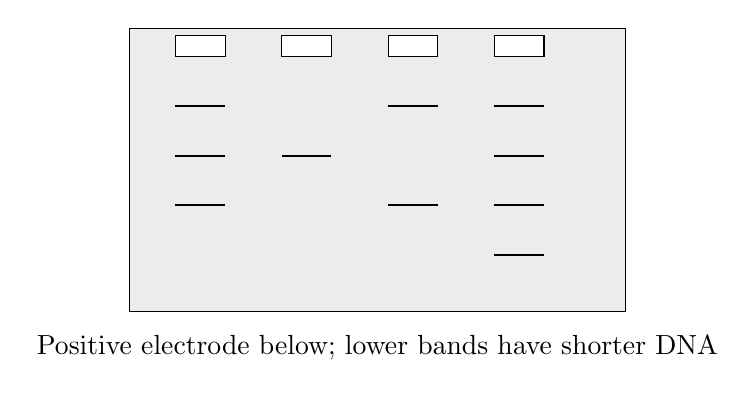
\begin{tikzpicture}[scale=0.9]
\draw[fill=gray!15] (0,0) rectangle (7,4);
\foreach \x in {1,2.5,4,5.5} {\draw[fill=white] (\x-0.35,3.6) rectangle (\x+0.35,3.9);}
\draw[thick] (0.65,2.9) -- (1.35,2.9);
\draw[thick] (0.65,2.2) -- (1.35,2.2);
\draw[thick] (0.65,1.5) -- (1.35,1.5);
\draw[thick] (2.15,2.2) -- (2.85,2.2);
\draw[thick] (3.65,2.9) -- (4.35,2.9);
\draw[thick] (3.65,1.5) -- (4.35,1.5);
\draw[thick] (5.15,2.9) -- (5.85,2.9);
\draw[thick] (5.15,2.2) -- (5.85,2.2);
\draw[thick] (5.15,1.5) -- (5.85,1.5);
\draw[thick] (5.15,0.8) -- (5.85,0.8);
\node at (3.5,-0.5) {Positive electrode below; lower bands have shorter DNA};
\end{tikzpicture}
\end{center}

This is a representation. Real gels are translucent; bands become visible under suitable light only after DNA-binding staining. DNA molecules are coiled chains, not little horizontal lines. Electrophoresis uses substantial voltage, and some dyes are harmful, so \textbf{only teachers or trained professionals should perform it in laboratories}; do not try it at home. You can, however, safely observe something sharing its first few preparation steps:

\begin{shiyan}
\textbf{Fishing DNA Out of Strawberries: A Home-Safety Version}

Materials: two or three ripe strawberries, a pinch of salt, a teaspoon of dish detergent, clean water, a sealable bag, gauze or coffee-filter paper, a clear glass, and chilled concentrated alcohol, such as chilled medical alcohol, with parental assistance and no ignition sources nearby.

Procedure: (1) Seal the strawberries in the bag after expelling air and mash them by hand, physically breaking cells. (2) Dissolve salt and detergent in just under half a glass of warm water, mix into the bag, and leave for ten minutes. Detergent disrupts the cell and nuclear membranes' lipid bilayers (Chapter 47); salt helps DNA aggregate. (3) Filter through gauze into the glass. (4) Slowly pour an equal volume of cold alcohol down the glass wall without stirring, then wait several minutes.

What to observe: white translucent clumps appear at the juice--alcohol interface and can be lifted with a toothpick. These contain thousands of tangled DNA strands mixed with some protein. DNA is insoluble in cold alcohol and precipitates from water.

Safety reminder: alcohol is flammable; avoid open flames throughout. None of the experimental materials may be eaten, and keep detergent out of eyes. Are the visible clumps one DNA molecule? (Hint: a single molecule is only two nanometers across.)
\end{shiyan}

\textbf{Translator safety note:} Alcohol handling requires direct adult supervision, eye protection, and separation from heat, sparks, and flames; never taste the mixture. Do not chill flammable alcohol in an ordinary household refrigerator or freezer. Have a qualified teacher select a safe preparation method or use a prepared demonstration. See \href{https://www.poison.org/articles/rubbing-alcohol-only-looks-like-water}{Poison Control alcohol guidance}, \href{https://ehs.stanford.edu/wp-content/uploads/Lab-Compliance-Cheat-Sheet.pdf}{Stanford flammable-storage precautions}, and \href{https://www.acs.org/education/celebrating-chemistry-editions/2024-ccew/science-safety-tips.html}{ACS activity safety}.

Gel electrophoresis does more than measure length: after PCR, a gel confirms amplification of the desired fragment, with a band only at the target length suggesting sound primer design. It also compares individuals' DNA differences and checks sample integrity. It remains everyday molecular-biology practice. Its most consequential use, however, is reading sequence itself.

\section{Sanger Sequencing: Revealing DNA at Dead Ends}

Now the central problem: how do we identify A, T, G, or C at every position in a several-hundred-letter DNA segment? No microscope can do it. Bases differ by only a few atoms, far below optical resolution, and electron microscopes cannot reliably distinguish all four. Direct looking fails, so DNA must \textbf{reveal its information indirectly}.

In 1977, the British biochemist Frederick Sanger developed a new method: \textbf{dideoxy chain-termination}, now known as Sanger sequencing. Recall Chapter 67: polymerase joins each new nucleotide to a hydroxyl at the growing chain's end. Sanger added a few altered nucleotides alongside the four ordinary kinds, lacking the hydroxyl needed for the next addition. Once incorporated, a dideoxynucleotide creates a \textbf{dead end}: the chain cannot extend and synthesis stops abruptly.

The key design labels each dideoxynucleotide with a different fluorescent color, one each for A, T, G, and C, then mixes them with ordinary nucleotides, polymerase, primer, and template. Since altered molecules are scarce, termination positions are random. One chain encounters a terminating A at position 50; another a terminating G at 51; another continues to a terminating C at 300. The completed reaction contains \textbf{new chains of many lengths}, each terminal color identifying why it stopped: a red end, for example, means termination at A.

These chains then undergo electrophoresis, actually through very fine quartz capillaries but using the same size-sorting principle. The shortest fragment, stopped after one added letter, reaches the detector first and is illuminated by a laser for color identification. Two-letter extensions follow, then three, and so on. The resulting color sequence translates to letters: first arrival identifies the first added base, second the second, and onward.

\begin{zhengju}
Sanger sequencing deserves a detailed story because it was not merely a flash of genius but a campaign to read invisible information.

Sanger had already accomplished something similar: during the 1950s, he spent ten years determining the sequence of all 51 amino acids in insulin, first demonstrating that proteins have definite sequences and earning the 1958 Chemistry Nobel Prize. If proteins could be sequenced, why not DNA? DNA had only four letters but thousands or tens of thousands in a chain, overwhelming protein sequencing's fragment-and-identify approach. By the 1970s, several laboratories were tackling it, mostly by breaking DNA into fragments, reading them, and reassembling, with slow progress.

Sanger changed perspective: instead of dismantling a long chain to read it, \textbf{make copying itself the reporter}. He first developed the plus-and-minus method and soon improved it into chain termination, exploiting polymerase's fidelity and susceptibility to trickery to convert sequence into fragment length plus terminal color, both measurable at the time. The paper appeared in 1977. Around the same time, Americans Maxam and Gilbert developed selective chemical cleavage at particular bases, also reading lengths by electrophoresis. The approaches competed and cross-checked one another, healthy science in action. Within years, chain termination prevailed: chemical cleavage required highly toxic reagents and cumbersome procedures, while chain termination was safe, simple, and automatable. Sanger earned his second Chemistry Nobel Prize in 1980.

The story continued with the Human Genome Project, launched in 1990 to read all roughly three billion human letters. The public effort first divided the genome into large mapped fragments, sequenced them, and assembled by landmarks, a reliable but slow approach. In 1998, entrepreneur Venter founded a company advocating whole-genome shotgun sequencing: randomly fragment everything, sequence it, and let computers assemble it. Public arguments over whether shotgun methods could handle extensive human repeats accelerated progress, and both sides released drafts in 2001. Later analyses showed that the public project's landmark data were crucial for resolving repeats. The competing approaches ultimately converged into today's standard practice.
\end{zhengju}

Sanger reads about 500--1,000 letters with high accuracy and remains a gold standard for validating short sequences. Yet it reads only one chain at a time. Reading a three-billion-letter human genome chain by chain requires enormous time and money. The Human Genome Project took about thirteen years and nearly three billion dollars. Reading more lives required a qualitative leap.

\section{High Throughput: A Million Chains at Once}

The leap came from a simple idea: \textbf{parallelism}. With one-chain chemistry established, read a million or a hundred million chains simultaneously.

Consider the most widely used sequencing-by-synthesis approach. Fragment sample DNA into one- or two-hundred-letter pieces and attach them densely to a glass chip, one cluster per position, like microscopic tufts of grass. Flow reagents across it so every cluster synthesizes DNA in synchrony. Here nucleotides carry fluorescent labels and a chemical shutter that pauses synthesis after every addition. At each pause, the instrument photographs the entire chip: each position's color identifies its newly incorporated base. Remove the label, resume synthesis, pause, and photograph again. After over a hundred cycles, each cluster's color history reveals its sequence.

A chip holds hundreds of millions of clusters, producing that many reads per run, even if each is only a little over a hundred letters. That is high throughput: short individual reads, enormous totals. Compare:

\begin{table}[htbp]
\centering
\begin{tabular}{lll}
\toprule
 & Sanger sequencing & High-throughput sequencing \\
\midrule
\shortstack[l]{Chains read\\at once} & 1 & \shortstack[l]{Tens to hundreds\\of millions} \\
Read length & 500--1,000 letters & 100--300 letters \\
Strength & \shortstack[l]{Precise validation\\of a short segment} & \shortstack[l]{Massive whole-genome\\coverage} \\
Typical use & Confirming a mutation & \shortstack[l]{Genomes and\\microbial communities} \\
\bottomrule
\end{tabular}
\end{table}

How dramatic is the effect? Reading a human genome cost hundreds of millions of dollars in 2001; by the 2020s, commercial prices fell to a few hundred dollars with completion in a day. Over twenty years, cost fell faster than computer chips' famous Moore's law. Sequencing moved from national projects to routine hospital testing: clinicians search tumor DNA for driver mutations, public-health teams trace viral transmission, and ecologists inventory life in seawater.

\section{Reassembling the Book: Errors and Bias}

High-throughput sequencing yields not a book but hundreds of millions of hundred-letter scraps. Restoring the book is \textbf{genome assembly}, a giant puzzle. If the last thirty letters of one scrap match the first thirty of another, they likely overlap neighboring genomic positions. Repeatedly overlapping and extending joins short pieces into long ones and eventually chromosomes.

Two formidable difficulties arise. First, \textbf{repeats}: over half the human genome consists of repeated passages, some identical sentences occurring thousands of times. If every chapter of a detective novel says ``It rained that night,'' a hundred-letter scrap may not reveal which chapter supplied it. The solution is to preserve clues: paired-end sequencing records both ends of the same longer fragment, retaining distance information. Newer long-read technologies instead produce scraps tens of thousands of letters long, spanning most repeats directly. Second, \textbf{errors}: each letter has roughly a one-percent chance of being read incorrectly because fluorescence imaging and chemistry are imperfect. What happens when a letter is wrong?

\begin{qiaoliang}
The answer is \textbf{read repeatedly and vote}. At a $1\%$ per-base error rate, one reading has a $1\%$ chance of error. But if thirty independent scraps cover a position, called 30-fold coverage, with unrelated errors, a wrong majority becomes negligibly unlikely. Roughly, at least sixteen of thirty making the same mistake has a probability below one in a trillion. Clinical human-genome sequencing therefore usually requires at least 30-fold coverage, using \textbf{redundancy} to outvote random error, not merely compensating for poor instruments. Conversely, at three- or four-fold coverage, one error may masquerade as a mutation, a classic interpretation pitfall.
\end{qiaoliang}

A subtler issue is \textbf{reference-genome bias}. In practice, researchers often avoid assembling the whole puzzle and align scraps against a reference genome, a standard answer, recording differences. This is fast, but large sequences present in your DNA and absent from the reference have nowhere to align and are discarded. More concerning, the first human reference mainly came from a few volunteers, about seventy percent from one person. Treating that as humanity's standard embeds bias: population-specific variants missing from it make those populations' data easier to misread. Scientists are constructing pangenome references from thousands of people's genomes to represent diversity better. Acknowledging that the standard answer itself changes is scientific honesty.

\section{Reading Letters Is Not Understanding Meaning}

The black box is now largely open: PCR amplifies targets, electrophoresis sorts lengths, termination and fluorescence reveal sequence, and computers assemble it. When do these techniques work or fail?

\begin{itemize}[itemsep=2pt]
\item Poor primers amplify wrong fragments or nothing at all, making electrophoretic verification indispensable.
\item Short reads fail to resolve highly repetitive regions, leaving assembly gaps.
\item Contamination, such as bacterial DNA, is faithfully sequenced too.
\item Low coverage lets sequencing errors mimic mutations.
\item Reference alignment misses large individual-specific structural differences.
\end{itemize}

\begin{wuqu}
``Technology is so advanced that reading a person's entire DNA gives the complete life manual, predicting diseases and personality.'' This is sequencing's commonest exaggeration. First, even the letters may be incomplete or wrong because of coverage, repeats, and reference bias. Second, even with perfect letters, \textbf{much of their meaning remains mysterious}. Only a little over one percent directly codes for proteins; much remaining sequence has unclear function. The same difference can matter greatly in one person yet show no effect in another because traits arise from interacting genes and environments (Chapter 73). Third, sequence has an additional layer of usage information: epigenetic marks (Chapter 74) influence which genes activate and how strongly, and sequencing cannot read these marks. DNA resembles an ancient book only one percent translated. Possessing the original is far from understanding it.
\end{wuqu}

\section{Back to the Saliva Tube}

We can now answer the opening question. Saliva contains shed oral-mucosal cells whose nuclei each contain a complete genome. A testing company extracts DNA, amplifies relevant segments hundreds of millions of times by PCR, or reads broadly using high-throughput sequencing, identifies letters at particular sites, and compares them with population databases. It then infers that a variant is more frequent in a certain population or associated with slower average caffeine metabolism.

Every step involves probability and statistics: amplification has efficiency limits, sequencing makes errors, alignment introduces bias, and final interpretation relies on population associations rather than individual laws. A report may provide interesting clues, but it has not seen through you and cannot do so.

The chain continues: reading helps us understand, and understanding soon raised a bolder question: can we \textbf{write}? Can we precisely change one letter or gene? That is next chapter's subject: gene-editing technology, its promise, and its restraints.

\begin{tiaozhan}
Why can short reads not resolve repeats? Suppose an identical sequence of length $L$ appears twice. If read length $r<L$, a read wholly inside the repeat has two indistinguishable origins, halting assembly. Only a read spanning the repeat and reaching unique single-copy sequence on both sides uniquely establishes position. Human genomes contain repeats hundreds of thousands of letters long with over $99\%$ similarity. No amount of hundred-letter coverage fills every gap: what is missing is not quantity but each scrap's field of view. Long reads increase $r$ by two orders of magnitude, bypassing this mathematical obstacle. Skipping this section will not lose the main thread, but it shows that sequencing limits often involve combinatorics, not chemistry alone.
\end{tiaozhan}

\section*{Try It Yourself}

\begin{sikaoti}
\item Draw three PCR cycles, using two lines for double-stranded template DNA and marking primer positions and directions. Count target copies after cycles one, two, and three. State that this is a representation and real DNA is not straight.
\item Why do longer negatively charged DNA fragments move more slowly in a gel? Explain how driving force and resistance from the mesh depend on length and which ultimately dominates.
\item Starting with 100 target molecules and 1.8-fold amplification per PCR cycle, estimate the count after twenty cycles. What if the starting count is ten? What initial-quantity information does the product count preserve?
\item Assemble these overlapping scraps: first = ...GATTACA, second = TACAGCC..., third = ...CAGCCAT. Write the combined sequence. If TACA occurs fifty times in the genome, is your assembly still reliable? Why?
\item A genetic report says your variant gives a disease risk 1.5 times the average. Using this chapter and Chapter 73, list at least three questions to ask before drawing conclusions. (Hints: coverage; correlation or causation; population or individual.)
\end{sikaoti}
